\documentclass[a4paper]{article}

\usepackage[pdftex]{graphicx}
\usepackage[margin=3cm]{geometry}
\usepackage{verbatim,moreverb,amssymb,amsmath}


\newcounter{question}
\newcommand{\question}[1]{\refstepcounter{question}\section*{Question~\thequestion~~~\small\emph{(#1)}}}
\renewcommand*\thequestion{\arabic{question}}


\begin{document}

\pagestyle{empty}
\thispagestyle{empty}



\noindent
\begin{minipage}{\columnwidth}
  \centering
  \Large
  DA4002 (HT11) Halmstad University\\
  Introduction to Algorithms, Data Structures, and Problem Solving\\[3\baselineskip]
  \Huge
  Written Exam\\
  \Large
  Thursday, August 22, 2013\\[2\baselineskip]
  Examiner: Roland Philippsen
\end{minipage}

\vfill

\noindent
\begin{center}
\fbox{
  \begin{minipage}{0.8\columnwidth}
    \textbf{Student Name:}\\[3\baselineskip]
  \end{minipage}
}
\end{center}

\vfill



\section*{Rules}

Aside from the obvious rules of conduct exams (e.g.\ no chatting):

\begin{itemize}
\item
  \textbf{No computing devices} (laptops, phones, calculators, \emph{etc}).
\item
  \textbf{No books or printouts} except for non-electronic dictionaries.
\item
  \textbf{Allowed hand-written notes}: two sheets of A4 paper (front and back).
\end{itemize}



\section*{General Guidelines}

\begin{itemize}
\item
  \textbf{Read carefully} and pace yourself.
  You can solve the problems in any order you want, but later problems may be easier to solve after you have answered the preceding questions.
\item
  \textbf{Write clearly} and draw clear diagrams.
  If you need to correct a mistake, then cleanly cross out the wrong answer and clearly indicate where the correction can be found.
\item
  \textbf{Indicate the question number} for each of your answers.
  If a question has sub-questions, indicate the sub-question number after the main question number, separated by a dot.
  For example, question 3 has 4 sub-questions, and their answers should be numbered 3.1, 3.2, 3.3, and 3.4.
\end{itemize}



\pagebreak
\pagestyle{plain}
\thispagestyle{plain}
\setcounter{page}{1}



\question{6 points}

\begin{enumerate}
\item
  Draw an example diagram for each of the following data structure types:
  \begin{enumerate}
  \item
    simply linked list
  \item
    doubly linked list
  \item
    binary tree
  \item
    directed acyclic graph
  \end{enumerate}
\item
  For each of the two following diagrams, explain why it is \textbf{not} a valid example of any of the above data structure types.
\end{enumerate}

\begin{center}
\fbox{(k-ary tree)}
\fbox{(directed cyclic graph)}
%%\includegraphics[width=0.4\columnwidth]{.pdf}
\end{center}


\clearpage


\question{5 points}

The following C code contains a tree data structure type declaration and three traversal functions.
Note that the \texttt{Fifo} data structure and the various \texttt{fifo\_} functions provide a first-in first-out queue whose implementation is not shown.

\begin{enumerate}
\item
  For each of the functions, write down whether it does pre-order, post-order, in-order, or level-order traversal.
\item
  Given the example tree in the diagram below, write down for each function the sequence of characters that it prints out.
  Note that the non-labeled horizontal arrows are the \texttt{sbl} pointers, the non-labeled downward-pointing arrows are \texttt{cld} pointers, and \texttt{\textsc{null}}-pointers are not shown.
\end{enumerate}

\vfill

\begin{minipage}[b]{0.65\columnwidth}
  \small
  \verbatimtabinput{q2-pseudocode.c}
\end{minipage}
\fbox{\begin{minipage}[b]{0.3\columnwidth}
    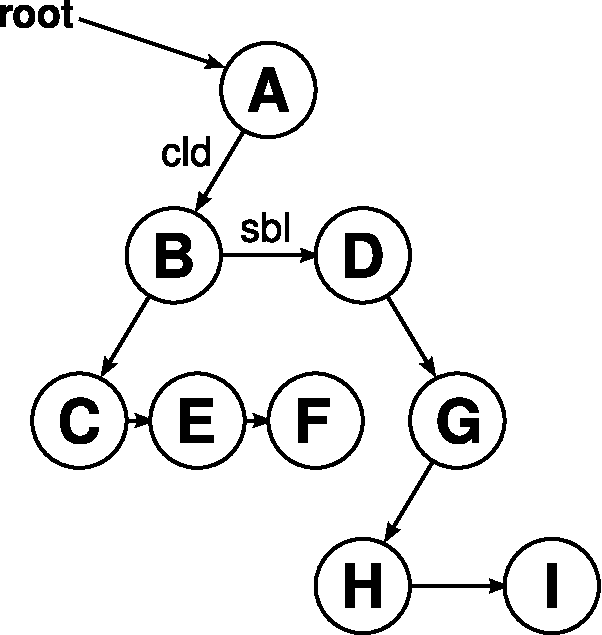
\includegraphics[width=\columnwidth]{q2.pdf}
\end{minipage}}

\end{document}
